\chapter{Requirements Analysis}\label{C:ra}
To guide the creation of the visualisation a user oriented design approach was
used, in particular making use of user models (personas). These personas were
created to give a sense of empathy and understanding for the foreseen users of
the visualisation in order to better understand the requirements and design
decisions to be made. 

The design of the visualisation was based heavily on User Centered Design as it
provided a method of user interface design as well as visualisation design. User
Centered Design is a process in which the needs, wants, and limitations of the
end users of a system are given extensive attention. To achieve this, personas
were created (also known as archetypal users), which are a personification the
needs of a larger group of related users. These personas act as stand-ins for
real users, describing them in terms of their goals and personal
characteristics, and although they are fictitious, they are based on knowledge
of real users. This design methodology supported my understanding of how users
were likely to use the visualisation.

An additional tool used during requirements analysis was User Scenarios which
describe the foreseeable interactions of the user personas with the
visualisation. A scenario is made up of a functional goal for the visualisation
and describes how it is carried out by a persona. Both of these tools force you
to think about the tasks needed for the visualisation and their context in the
system as a whole. Once the personas and scenarios have been completed you can
then start to design specific elements of the user interface and visualisation
based on the requirements and interactions described in the scenarios.
\section{User models}
Below are the two personas that were used in the design of the visualisation for
this project. They depict users that would use the visualisation in the context
of a terminal or display in an observatory environment. These personas  can be
validated during evaluation of the visualization by finding real users that
match the core values of the personas.

\subsection{John Truman (Primary Persona - The interested layperson)}\
24 year old John is interested in planets and space and has a basic knowledge
about both. He frequently visits attractions catering to this interest at
locations such as planetariums and observatories. Some of his favourite things
to do when visiting these attractions is to go to the computer terminals that
allow users to choose what information they see.

John is used to playing computer games and using visualisations and is not
overwhelmed understanding and using new systems. He finds that he learns better
when provided with visual examples than when reading or listening to
information. John is most comfortable using keyboard and mouse when interacting
with a computer.
\subsection{Cara Thompson (Secondary Persona - Likes gesture based systems)}
23 year old Cara likes using interactive visualisations when visiting
attractions, she finds that they are more entertaining and provide a better
level of interaction and more of a novelty experience with a visualisation than
simply a keyboard and mouse. 
\\\\
Both of these users are similar in their need for information from the
visualisation but differ in the methods that they wish to access the information
and interact with the visualisation. John wants to interact with keyboard and
mouse as it is more straight forward and accurate. Cara wants to interact with
gestures as she finds it more of a novelty and more immersive.
\section{Scenarios}
 A good use scenario does a number of things:
\begin{itemize}
 \item Describes the user's goals and motivations.
  \item Describes a specific task or tasks that need to be accomplished.
   \item Describes some of the interaction, with enough detail to make it
compelling, but not so much detail as to be overwhelming.
    \item Provides a shared understanding for everyone on your team about what a
user might want to do and how they might do it.
     \item Helps you construct the sequence of events that are necessary to
address in your user interface.
     \item Can be sketchy, as long as it provokes ideas and discussion.
\end{itemize}
 \subsection{Scenario 1: View planets ordered by their similarity to Earth}
   {\bf Primary Persona:}\\
 When John first sees the system the first thing he notices is that their are
many planets orbiting what looks like a star. He doesn't have any point of
reference for these planets so their sizes, colours, and movement speeds are
meaningless. By providing a way of comparing the planets to Earth it gives a
point of reference which is well documented and known by most.
 
 {\bf Procedure:}
 \begin{enumerate}
 \item John clicks a prominent button stating view planet similarity to earth.
 \item The planets on screen move so that the earth is located at the center and
top of the screen with all others orbiting it. The planets with a high internal
similarity to earth are higher on the Y axis whilst the planets with a high
surface similarity to earth are closer to the center of the orbiting planets on
the X axis.
 \item From here John can select any of the planets for further analysis.
 \end{enumerate}
 \subsection{Scenario 2: Select ranges for attributes of each planet displayed}
   {\bf Primary Persona:}\\
 John has become comfortable with selecting the planets and has some idea of the
scale and basic attributes of the planets. Now he wants to select more planets
to find out more information. However due to the large number of planets he
finds it difficult to accurately select them due to overlapping and fast moving
small planets.
 
  {\bf Procedure:}
  \begin{enumerate}
 \item John uses a range of filters to remove planets from his view that don't
match the criteria he chooses (temp ,size ,KOI , ESI).
\item As planets disappear the graph of planets expands into the space that
frees up, this causes more space to appear between planets making them more
selectable.
 \end{enumerate}
 \subsection{Scenario 3: Select planets to display more information}
  {\bf  Primary Persona:}\\
 John wants to see more information about each of the planets he can see
orbiting in the visualisation. To do this he wants to be able to select the
planets and have textual information appear on screen.
 
  {\bf  Procedure:}
   \begin{enumerate}
 \item John has the option to pause the rotation of planets in order to make
more accurate selections. 
 \item John clicks on a planet orbiting a planet.
\item The planet selected becomes larger and its outline grows, making it more
visible.
\item The text window has all of the information about the planet selected added
to it.
 \end{enumerate}
   {\bf  Secondary Persona:}\\
 Cara wants to see more information about each of the planets she can see
orbiting in the visualisation. To do this she wants to be able to hover her hand
over a planet to get the information to display on screen.
 
  {\bf  Procedure:}
   \begin{enumerate}
 \item Cara hovers her hand over a planet to make a selection
 \item The planet selected becomes larger and its outline grows, making it more
visible.
\item The text window has all of the information about the planet selected added
to it.
 \end{enumerate}
 \subsection{Scenario 4: View planets in the same solar system}
   {\bf  Primary and Secondary Personas:}\\
John and Cara are curious about which of the planets they can see in the
visualisation are in the same Solar System. To discover this they want that when
a planet is selected all other planets in the same Solar System as the selected
planet to become highlighted.
 
  {\bf  Procedure:}
   \begin{enumerate}
 \item When a planet is selected, all planets in the same Solar System become
larger and its outline grows, making it more visible.
 \item A label appears on these planets indicating that they are related
planets.
 \end{enumerate}
 \subsection{Scenario 5: View the Goldilocks zones of each planet}
   {\bf  Primary Persona:}\\
   Looking at the planets orbiting the sun in the viusalisaiton John wonders
whether any of them could support life. To see this John wants to see which
planets are in the habitable zones of their stars. 
 
  {\bf  Procedure:}
   \begin{enumerate}
 \item John clicks a button saying "Show habitable zones"
 \item Coloured rings appear showing the cold (blue), habitable (green), and hot
(red) zones of the selected planets star.
 \item When a planet from a different star system is clicked the coloured rings
will change to that stars zones.
 \end{enumerate}
 \subsection{Scenario 6: Select two planets to compare against one another}
    {\bf  Primary Persona:}\\
When John is selecting planets to view more information he often finds that he wants to compare his selections against another planet. To do this John wants to be able to make multiple selections to compare two planets against one another.
  
  {\bf  Procedure:}
   \begin{enumerate}
 \item When John selects a planet a button becomes ungreyed called "Compare"
with a note next to it saying "Please select another planet to compare to".
 \item When the second planet is selected a second text box fills up with the
information about the second planet. This information can be compared with that
in the first text box.
  \end{enumerate}
  
 \subsection{Scenario 7: Navigate the visualisation with gestures}
    {\bf  Secondary Persona:}\\
Cara doesn't find using keyboard and mouse interesting enough for interacting with the visualisation. She would rather navigate around the visualisation by using hand
gestures as it's more immersive.

  {\bf  Procedure:}
   \begin{enumerate}
 \item By moving her hand to the edges of the screen the visualisation with pan
in the correstponding direction, ie if the hand goes to the top of the screen
the visualisation pans up.
 \item By moving her hand backwards and forwards the visualisation will zoom in
and out.
  \end{enumerate}
\section{Requirements summary}
\subsection{Functional Requirements}
Functional requirements define the functions of a system. These functions are
described as a set of inputs, the behavior, and outputs from the system. The functional requirements for this visualisation are as follows:
\begin{enumerate}

 \item[R1.] The visualisation needs to display planetary information to convey
knowledge to users.
 \item[R2.] The planets need to be able to be ordered by their similarity to
earth (ESI) and by their Kepler Object of Interest number (KOI).
 \item[R3.] The visualisation needs to allow users to define ranges of planetary
attributes to filter which planets are displayed.
 \item[R4.] All planets need to be selectable and react appropriately when
clicked.
 \item[R5.] When a planet is selected all other planets in the same solar system
need to become more visible.
 \item[R6.] There needs to be the option to view the habitable zones of stars
and show where the planets orbiting them are in relation.
 \item[R7.] The visualisation needs to allow exoplanets to be compared against
one another.
\end{enumerate}


\subsection{Nonfunctional Requirements}
 Functional requirements are supported by non functional requirements. Non
functional requriements impose constraints on the design or implementation (such
as performance, security, or usability) of a system.
 
 The non functional requirements for this visualisation are as follows:
\begin{enumerate}
 \item[R8.] The visualisation needs to have a range of interactive buttons for
each element of interactivity in the system to help inform users how to use the
system.
 \item[R9.] All interaction methods must be visible and intuitive.
 \item[R10.] The visualisation needs to display attributes of each of the
Exoplanets.
 \item[R11.] The visualisation must remain uncluttered.
 \item[R12.] The visualisation must not show so much information that it causes
information overload for users.
  \item[R13.] There needs to be two modes of interaction with the system,
keyboard and mouse vs gesture based.
\end{enumerate}

%matrix
\begin{figure}[h!]
  \centering
      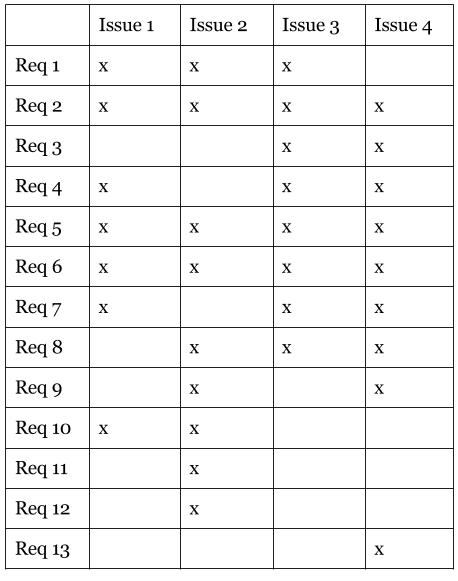
\includegraphics[width=0.8\textwidth]{images/issues_to_req_matrix.jpg}
  \caption{Matrix of project requirements to issues project is attempting to
address}
\end{figure}
